\subsection{Uncalibrated}

\subsubsection{Sol-185}

This sol was selected by us for reconstruction as it was recogonized as a region of interest with with unique geological makeup. Which led to make the rover spending more time in the area by taking many high quality images using the Mastcam. Arround 108 images were used to reconstruct the scene form sol 180 to sol 188. Thus having multiple view of images provided to be an advantage during reconstruction.

\begin{figure}[H]
	\centering
	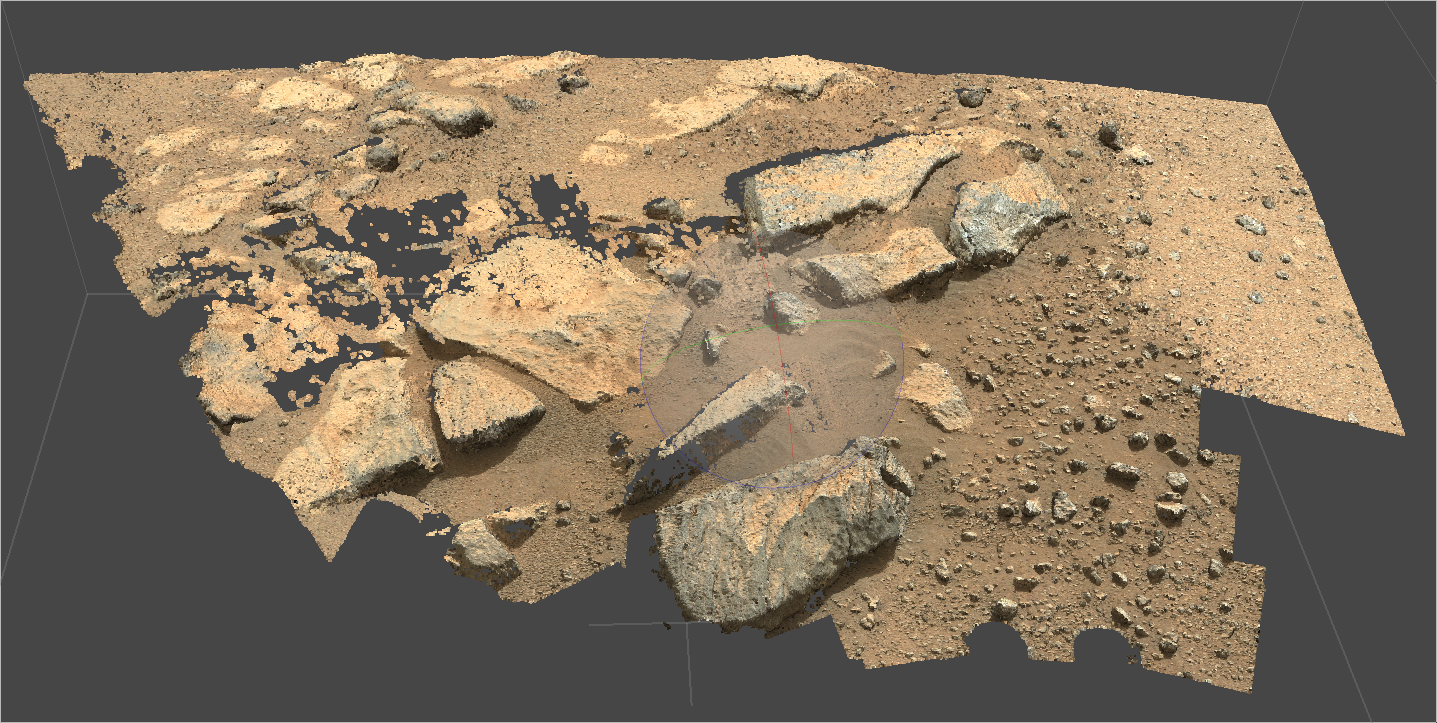
\includegraphics[scale=0.3]{img/sol185.png}
	\label{fig:sol185}
	\caption{}
\end{figure}

\subsubsection{Sol-197}

This rock is named "Rochette" by NASA, as they decided to drill a second time on this rock since it had unique features and geological makeup which was an interest for astrobiology. Thus providing us with 35 Mastcam images of high quality for the reconstruction. The images from sol 197 and sol 198 were used which are the images post boring on the rock. 


\begin{figure}[H]
	\centering
	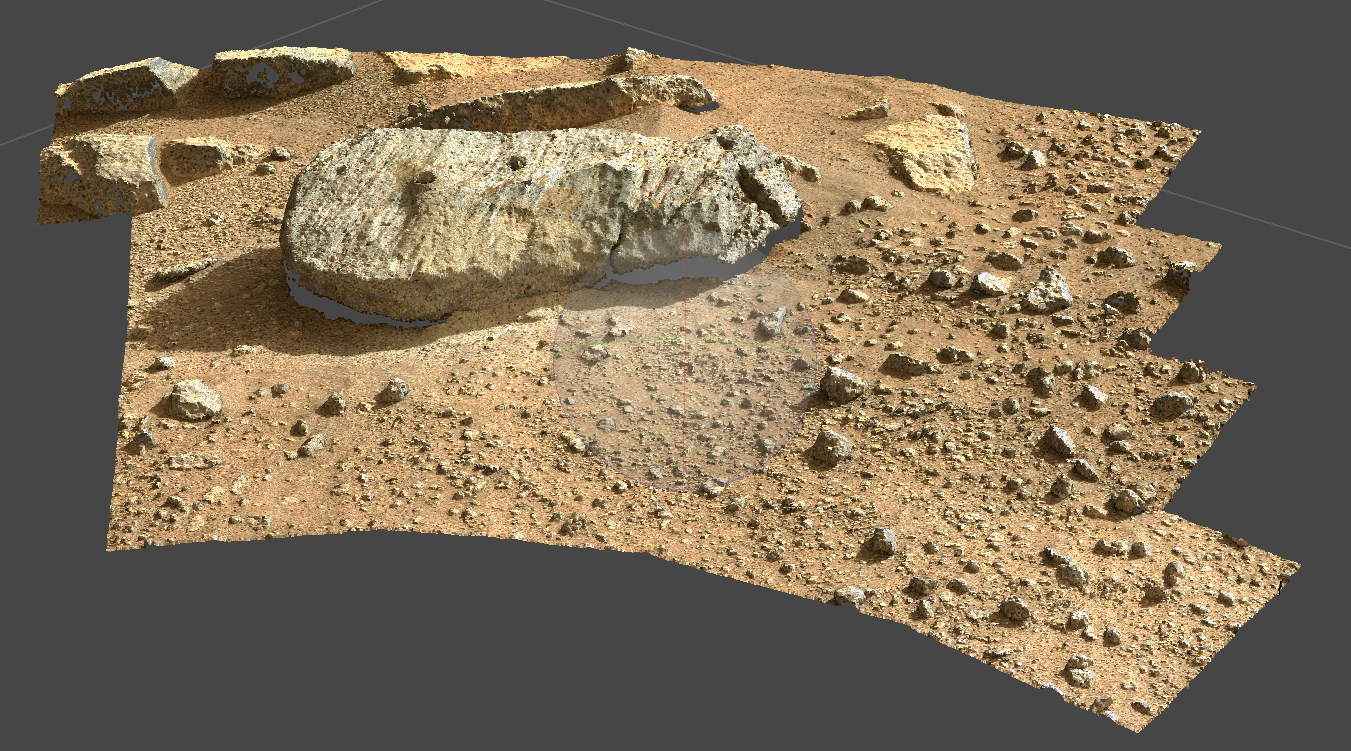
\includegraphics[scale=0.3]{img/sol195.png}
	\label{fig:sol197}
	\caption{}
\end{figure}

\subsubsection{SOl-106}

This location was reconstructed using 118 images. We used the high quality Mastcam images form sol106.

\begin{figure}[H]
	\centering
	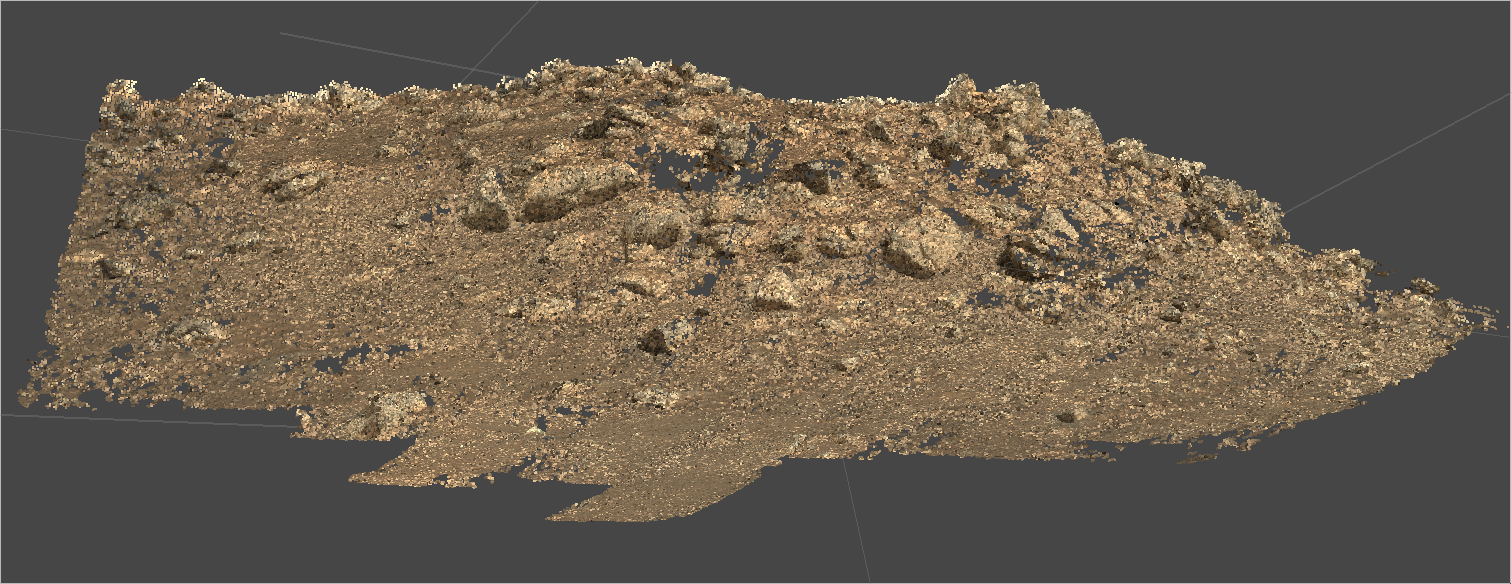
\includegraphics[scale=0.3]{img/sol106pc.png}
	\label{fig:sol103}
	\caption{}
\end{figure}

\subsubsection{Sol-268}
\label{sec:drilluncal}

This location was used to collect a sample for geological purpose. The reconstructed part potrays the drill that was made by the rover. We used 4 images from different angles form Mastcam to give a quality reconstruction.

\begin{figure}[H]
	\centering
	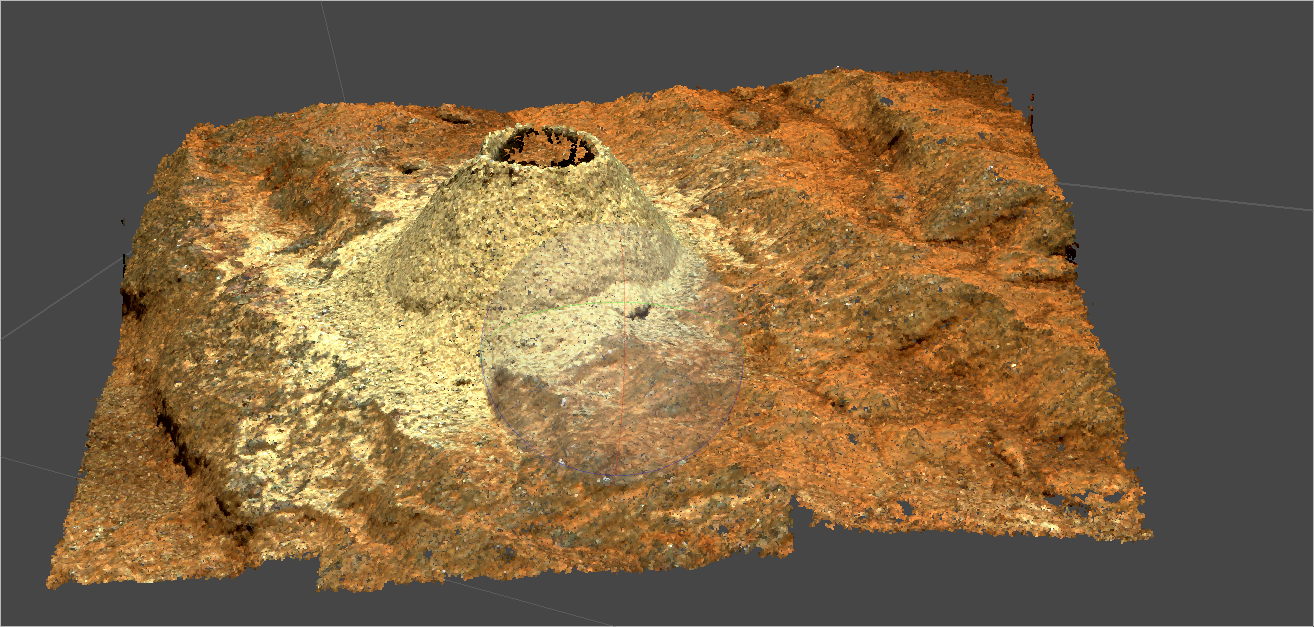
\includegraphics[scale=0.3]{img/sol286.png}
	\label{fig:sol268}
	\caption{}
\end{figure}

\subsubsection{Sol-54}
\label{sec:sol54}

The location had more high quality photos for reconstruction. We used 118 images from the Mastcam to reconstruct the area. 

\begin{figure}[H]

	\centering
	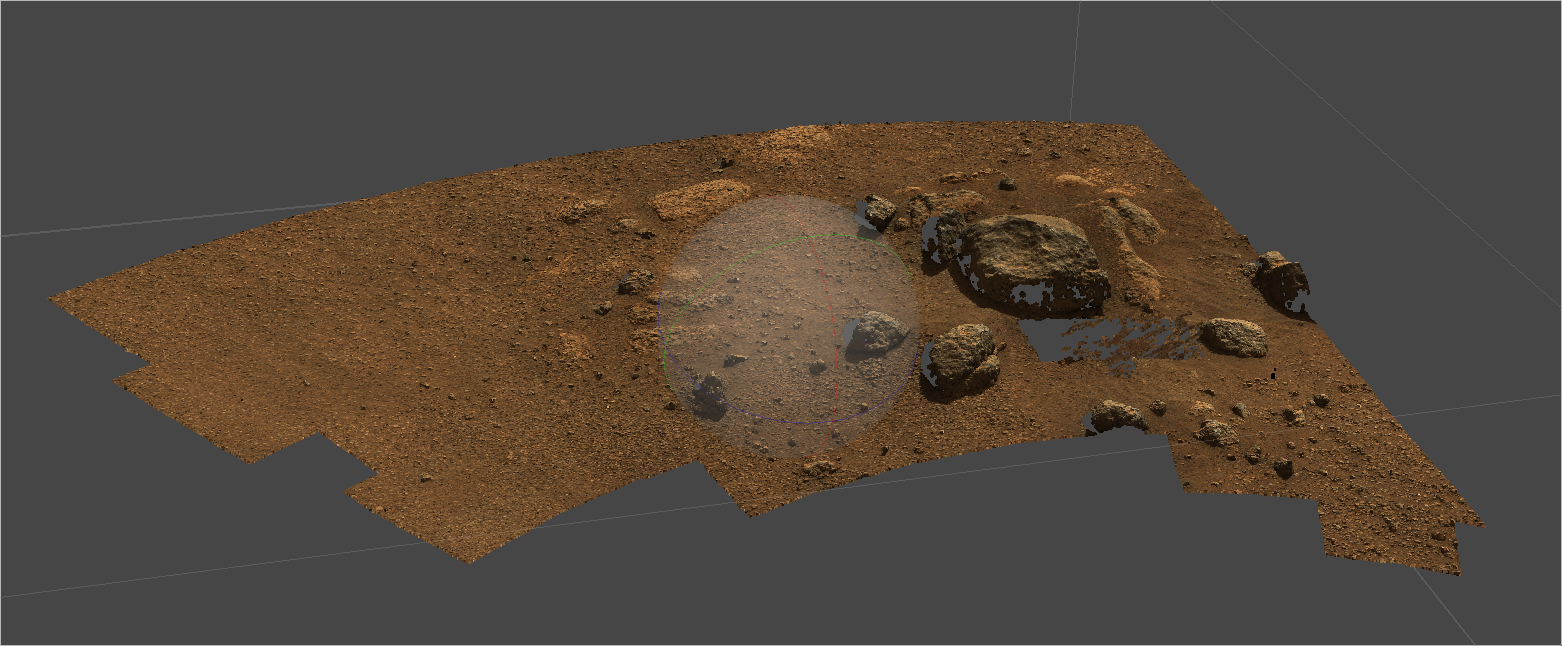
\includegraphics[scale=0.3]{img/sol42.png}
	\label{fig:sol54}
	\caption{}
\end{figure}
\subsubsection{Sol-283}

This location is one of newer area which the rover was exploring at the time, which had many features. This reconstruction was done by us using 8 images from the Mastcam.
\begin{figure}[H]
	\centering
	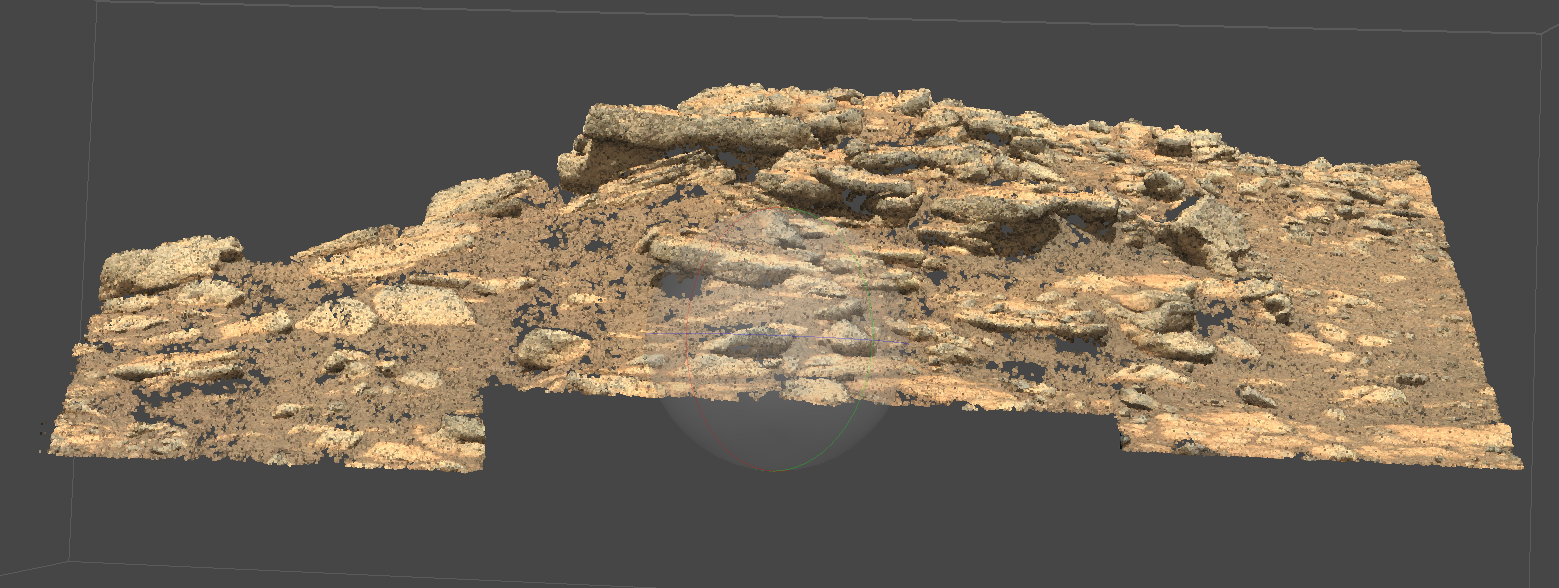
\includegraphics[scale=0.3]{img/sol2283.png}
	\label{fig:sol283}
	\caption{}
\end{figure}

\subsection{Callibrated}

\subsubsection{Sol-268}

Reconstruction of a drill made by rover with 4 Mastcam images. We included the parameters for the images which gave a good reconstruction and to produce an actual scale of the region unlike in \ref{sec:drilluncal}. Including the extrinsics gives the correct orientation of the area and the location of the object.

\begin{figure}[H]
	\centering
	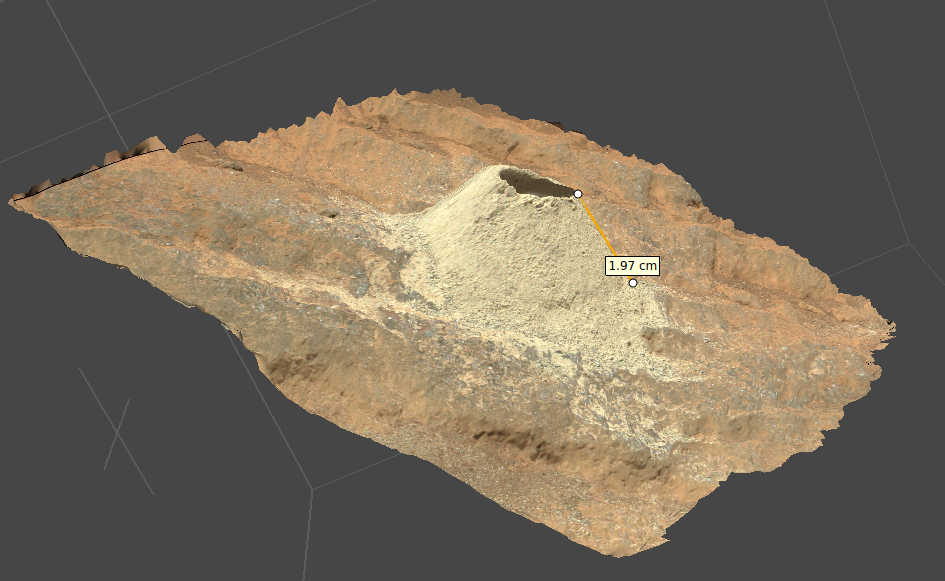
\includegraphics[scale=0.3]{img/drill.png}
	\label{fig:sol268calib}
	\caption{}
\end{figure}
\subsubsection{Sol-54}

In this Reconstruction of sol 54 we included the intrinsic and the extrinsics parameters in the agisoft with the same number of images as \ref{sec:sol54}. This gave us the correct orientation of the area.


\begin{figure}[H]
	\centering
	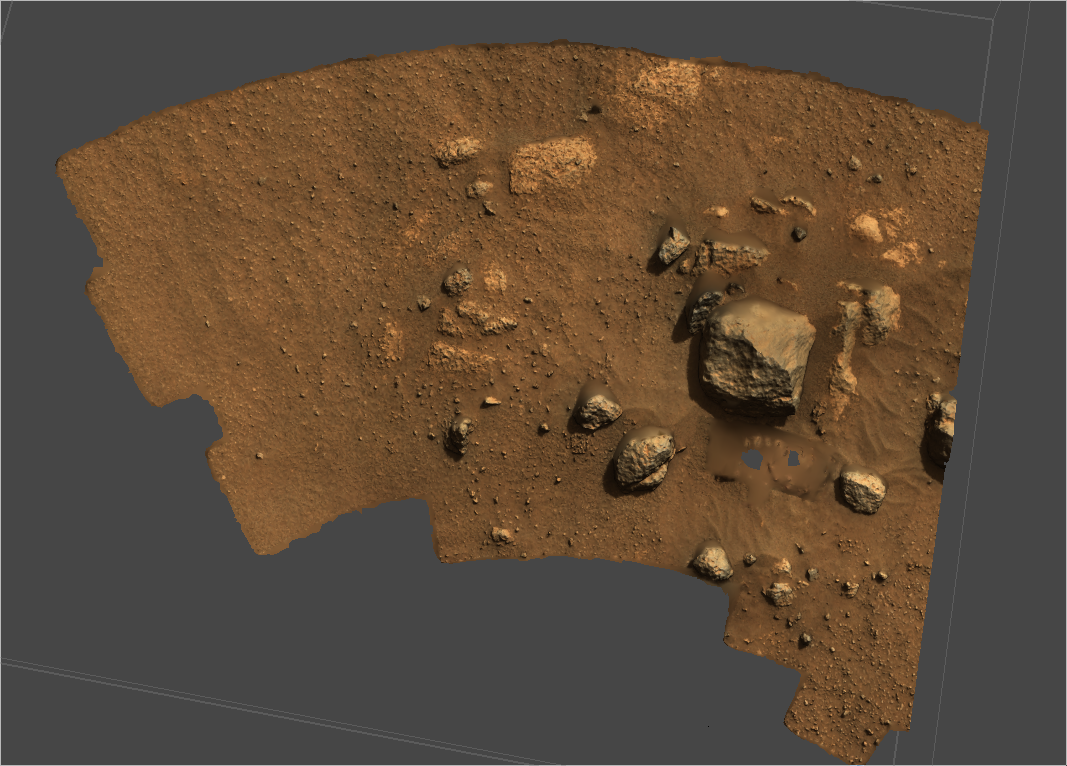
\includegraphics[scale=0.3]{img/sol54calib.png}
	\label{fig:sol54calib}
	\caption{}
\end{figure}

\subsubsection{Sol-283}

This sol was a considerably newer region which the rover was set to explore. Comparing with the Uncalibrated reconstruction the orientation in the Callibrated reconstruction was more accurate. We used 8 images from the Mastcam for the reconstruction. 


\begin{figure}[H]
	\centering
	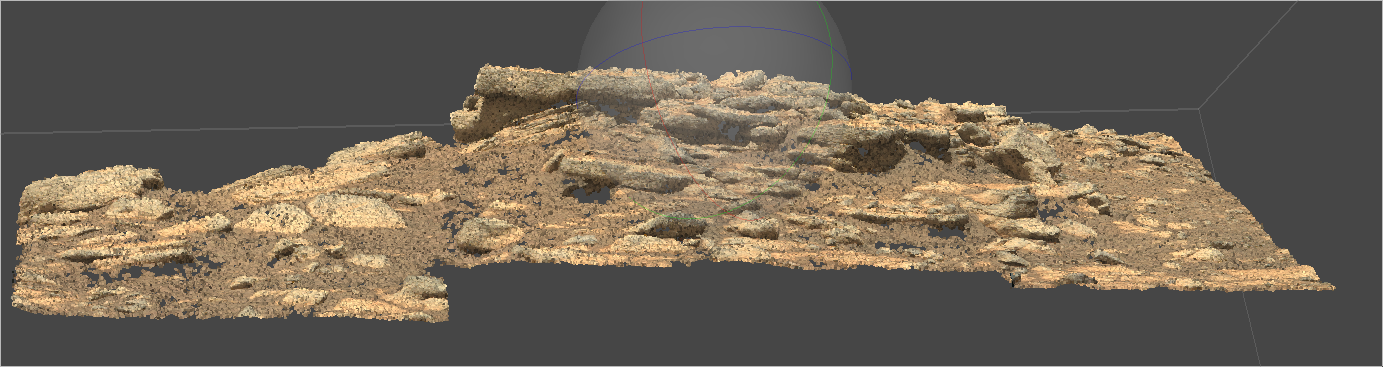
\includegraphics[scale=0.3]{img/sol283calib.png}
	\label{fig:sol283calib}
	\caption{}
\end{figure}
